%\documentclass[pt12]{beamer}
\PassOptionsToPackage{dvipsnames}{xcolor}
\documentclass[10pt,externalviewer]{beamer}

\usepackage[dvipsnames]{xcolor}
\usepackage{amssymb}
\usepackage{rotating}
\usepackage{amsmath}
\usepackage{hyperref}
\usepackage{bookmark}
\usepackage{bigints}
\usepackage{graphics}
\usepackage{natbib}
\usepackage{caption}
\usepackage{subcaption}
\usepackage{tikz}
\usepackage{lipsum}
\usepackage[italian]{babel}
\usepackage[utf8]{inputenc}
\usepackage[T1]{fontenc}
\usepackage[mode=math]{siunitx}
\usepackage[absolute,overlay]{textpos}
\usepackage{pdfcolparallel}
\usepackage{tcolorbox}
\usepackage{physics}
\tcbuselibrary{fitting}

\makeatletter
\newcommand\xleftrightarrow[2][]{%
  \ext@arrow 9999{\longleftrightarrowfill@}{#1}{#2}}
\newcommand\longleftrightarrowfill@{%
  \arrowfill@\leftarrow\relbar\rightarrow}
\makeatother

\definecolor{PDred}{HTML}{9B0014} % Catania green (primary)

\mode<presentation>
{
  \usetheme{Warsaw} 
%  \usetheme{Madrid}
%  \usetheme{Montpellier}
%  \usetheme{Marburg} 
  \usecolortheme[named=PDred]{structure}
  \setbeamercolor{alerted text}{fg=PDred}
  \setbeamercovered{transparent}
  \setbeamertemplate{section in toc}[ball unnumbered]
  \usefonttheme[]{serif}
  \setbeamerfont{author}
  {size=\scriptsize,parent=structure}
  \setbeamerfont{date}
  {parent=structure}
  \setbeamerfont{title}
  {size=\Large,parent=structure}
  \setbeamerfont{sectiontitle}
  {size=\Large,parent=structure}
}

%\setbeamertemplate{footline}{\hfill\insertframenumber/\inserttotalframenumber} 

\expandafter\def\expandafter\insertshorttitle\expandafter{%
  \insertshorttitle\hfill%
  \insertframenumber\,/\,\inserttotalframenumber}

\newcommand{\backupbegin}{
   \newcounter{framenumberappendix}
   \setcounter{framenumberappendix}{\value{framenumber}}
}
\newcommand{\backupend}{
   \addtocounter{framenumberappendix}{-\value{framenumber}}
   \addtocounter{framenumber}{\value{framenumberappendix}} 
}

\newcommand{\refer}[1]{%
   \begin{flushright}
      {\alert{\tiny #1}}
   \end{flushright}}
  
\newcommand{\lrefer}[1]{%
   \begin{flushleft}
      {\alert{\tiny #1}}
   \end{flushleft}}
  
\newcommand{\param}[1]{%
   \begin{flushright}
      {\small #1}
   \end{flushright}
   \vspace{-1.5\baselineskip}
}

%\newcommand{\sech}{\mathop{\rm sech}\nolimits}
\newcommand{\sgn}{\mathop{\rm sgn}\nolimits}
\newcommand{\etal}{{\em et al.}}


\title{Simulation and Analysis of 1D Wave Propagation under Various Physical Models}

\author[Dario Liotta]{\large{\textbf{Dario Liotta}}}

\institute[Physics of Data (UniPD)]{
\begin{minipage}[c]{3.4truecm}

\includegraphics[width=\textwidth]{logo-unipd}
\end{minipage}
\begin{minipage}[c]{2truecm}
   \begin{flushleft}
   \end{flushleft}
\end{minipage}
\begin{minipage}[c]{4.2truecm}

\includegraphics[width=\textwidth]{logo-dfa}
\end{minipage}}

\date{September 6th 2025 \\ Course of \textbf{Quantum Information and Computing} \\ Academic Year 2024/2025}

\begin{document}

\begin{frame}[plain]
\titlepage
\end{frame}

\section{Finite Element Method}

\begin{frame}
   \frametitle{Building up the workspace: the setup}

   First I created a \textcolor{BrickRed}{\textbf{working directory}}

   \begin{figure}[H]
      \centering
      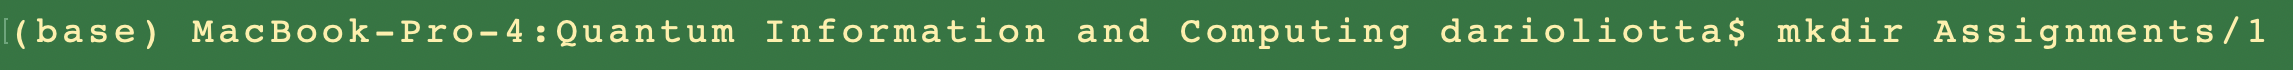
\includegraphics[width=\textwidth]{Immagini/creating-working-directory.png}
   \end{figure}

   \vfill

   \begin{minipage}{0.45\textwidth}

      \begin{center}
         The \textcolor{BrickRed}{\textbf{development environment}} I chose
      \end{center}

      \vspace{-0.5cm}

      \begin{figure}[H]
         \centering
         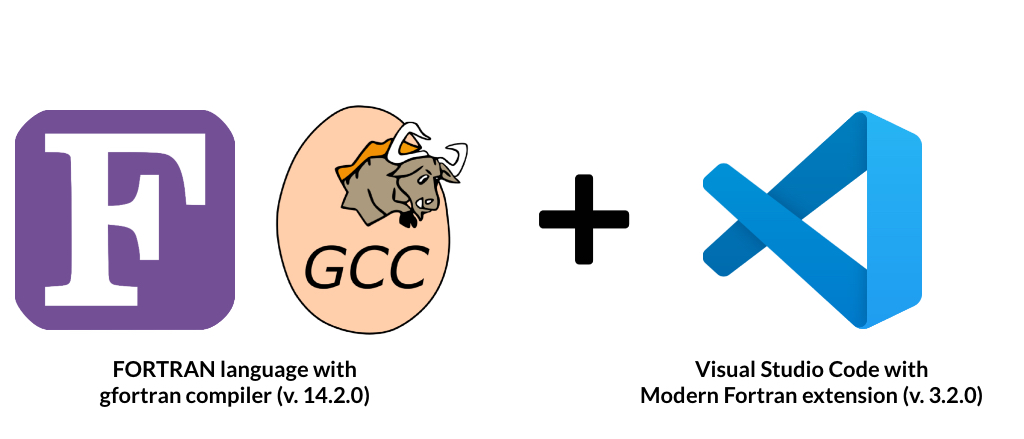
\includegraphics[width=\textwidth]{Immagini/setup.jpg}
      \end{figure}

   \end{minipage}
   \hfill
   \begin{minipage}{0.45\textwidth}

      \begin{center}
         Finally, I submitted the simplest program: \textcolor{BrickRed}{\textbf{\texttt{hello\_world.f90}}}
      \end{center}

      \begin{figure}[H]
         \centering
         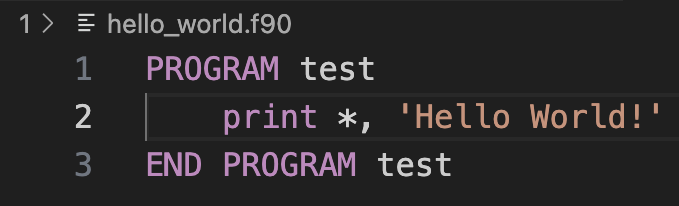
\includegraphics[width=0.65\textwidth]{Immagini/hello_world_code.png}
         \caption*{\scriptsize{\textbf{Code}}}
      \end{figure}

      \vspace{-0.6cm}

      \begin{figure}[H]
         \centering
         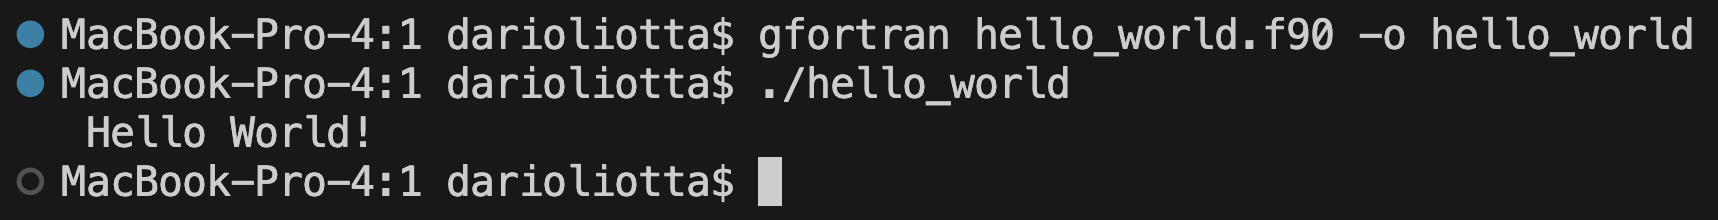
\includegraphics[width=\textwidth]{Immagini/hello_world_output.png}
         \caption*{\scriptsize{\textbf{Output}}}
      \end{figure}

   \end{minipage}
\end{frame}

\section{Number precision}

\begin{frame}
   \frametitle{Exploring the limits of INTEGER and REAL in Fortran}

   \begin{minipage}{0.45\textwidth}

      \begin{center}
         \textbf{Sum of integers}

         \vspace{-0.5cm}

         \scriptsize{$$\num{2000000}+1$$}
      \end{center}

      \footnotesize{In Fortran we can select how much space we give to our variables:}

      \begin{itemize}
         \footnotesize{\item \textcolor{BrickRed}{\textbf{\texttt{INTEGER*2}}}: \textbf{2 bytes} $\Rightarrow$ 16 bits $\Rightarrow \ n\in\left[-2^{15},2^{15}-1\right]$}
         \footnotesize{\item \textcolor{BrickRed}{\textbf{\texttt{INTEGER*4}}}: \textbf{4 bytes} $\Rightarrow$ 32 bits $\Rightarrow \ n\in\left[-2^{31},2^{31}-1\right]$}
      \end{itemize}

      \begin{center}
         \footnotesize{$\num{2000000}>2^{15} \ \Rightarrow$} \textcolor{BrickRed}{\textbf{Compiler error}}
      \end{center}

      \vspace{-0.25cm}

      \begin{figure}[H]
         \centering
         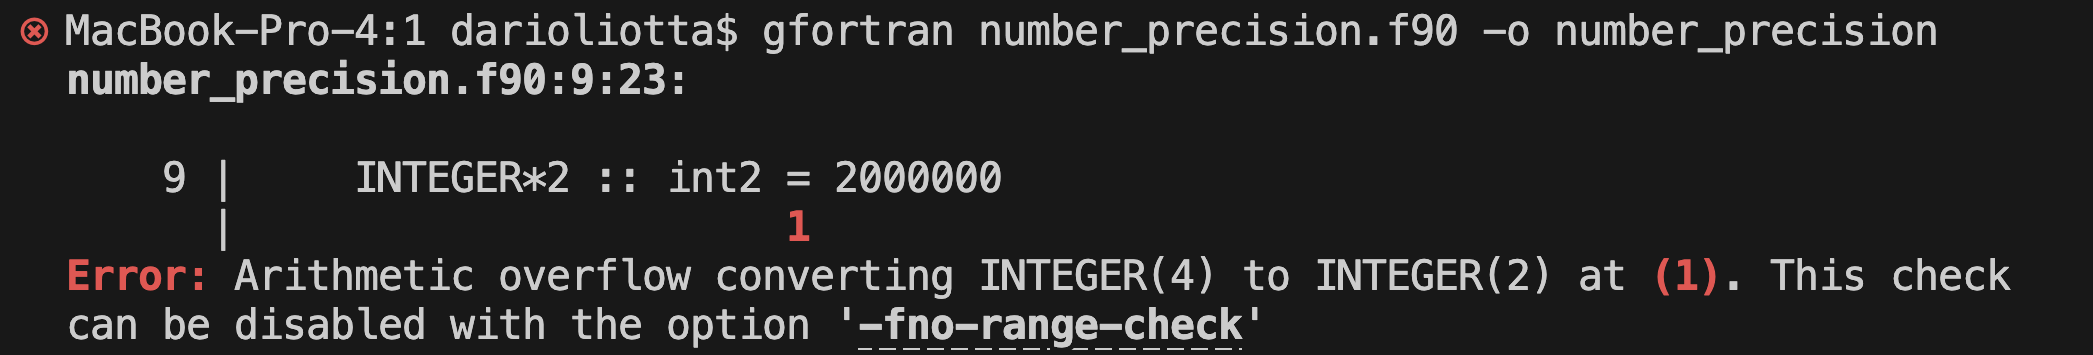
\includegraphics[width=\textwidth]{Immagini/integer_sum_error.png}
      \end{figure}

      \footnotesize{Forcing with the \texttt{-fno-range-check} flag results in an \textcolor{BrickRed}{\textbf{overflow}}}

      \begin{figure}[H]
         \centering
         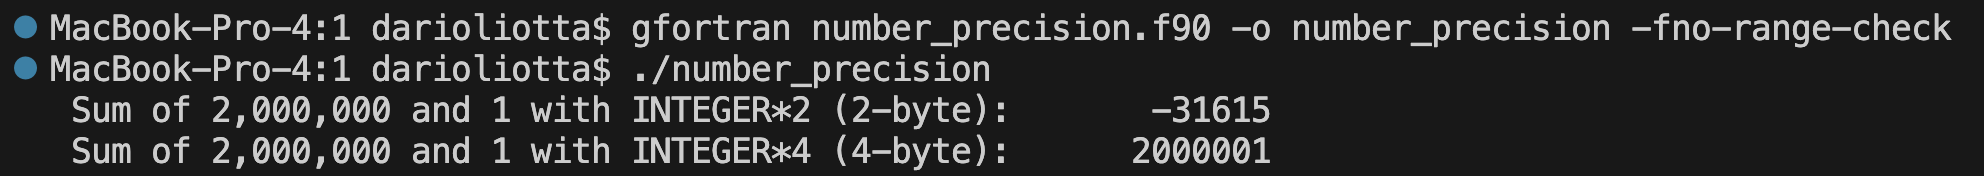
\includegraphics[width=\textwidth]{Immagini/integer-sum-output.png}
      \end{figure}

   \end{minipage}
   \hfill
   \begin{minipage}{0.45\textwidth}

      \begin{center}
         \textbf{Sum of reals}

         \vspace{-0.5cm}

         \scriptsize{$$\pi\cdot10^{32}+\sqrt{2}\cdot10^{21}$$}
      \end{center}

      \footnotesize{Different storage lengths mean different precisions:}

      \begin{itemize}
         \footnotesize{\item \textcolor{BrickRed}{\textbf{Single}}: \textbf{4 bytes} $\Rightarrow$ 32 bits\\ $\Rightarrow$ up to $8$ decimal digits}
         \footnotesize{\item \textcolor{BrickRed}{\textbf{Double}}: \textbf{8 bytes} $\Rightarrow$ 64 bits\\ $\Rightarrow$ up to $16$ decimal digits}
      \end{itemize}

      \vspace{-0.25cm}

      \begin{figure}[H]
         \centering
         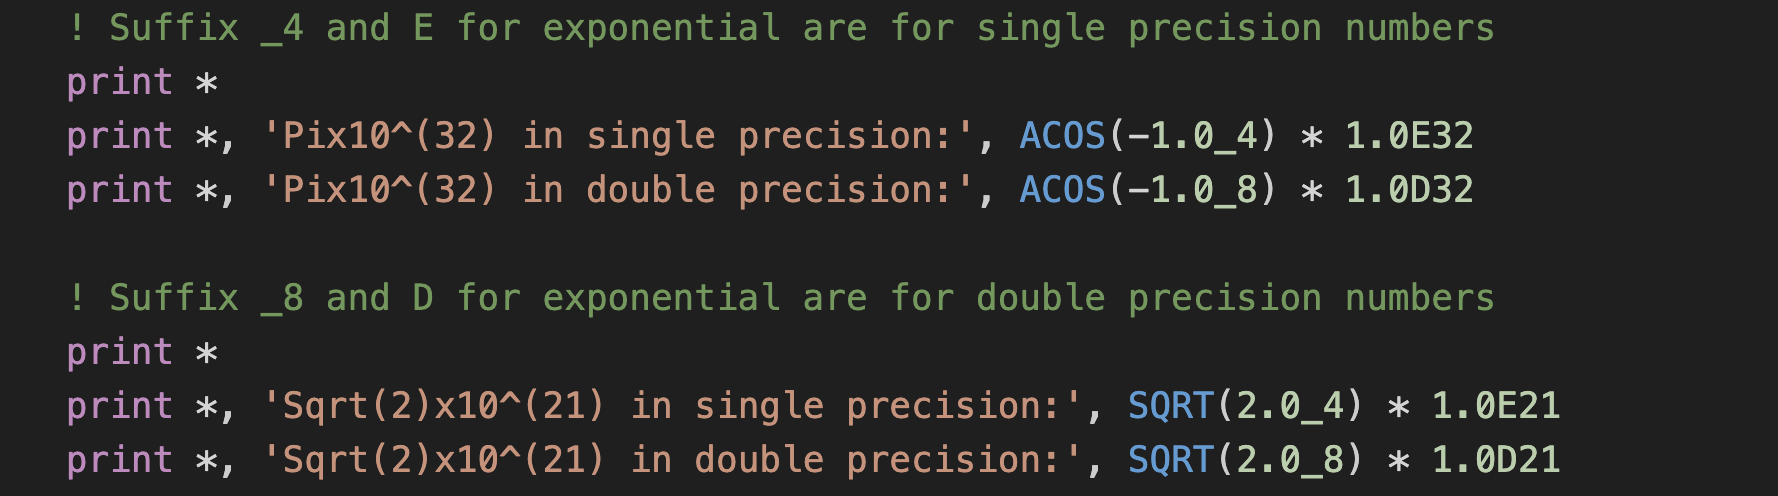
\includegraphics[width=0.78\textwidth]{Immagini/real-sum-code.png}
      \end{figure}

      \footnotesize{A difference of $11$ orders of magnitude means \textcolor{BrickRed}{\textbf{no difference}} in single precision from $\pi\cdot10^{32}$}

      \begin{figure}[H]
         \centering
         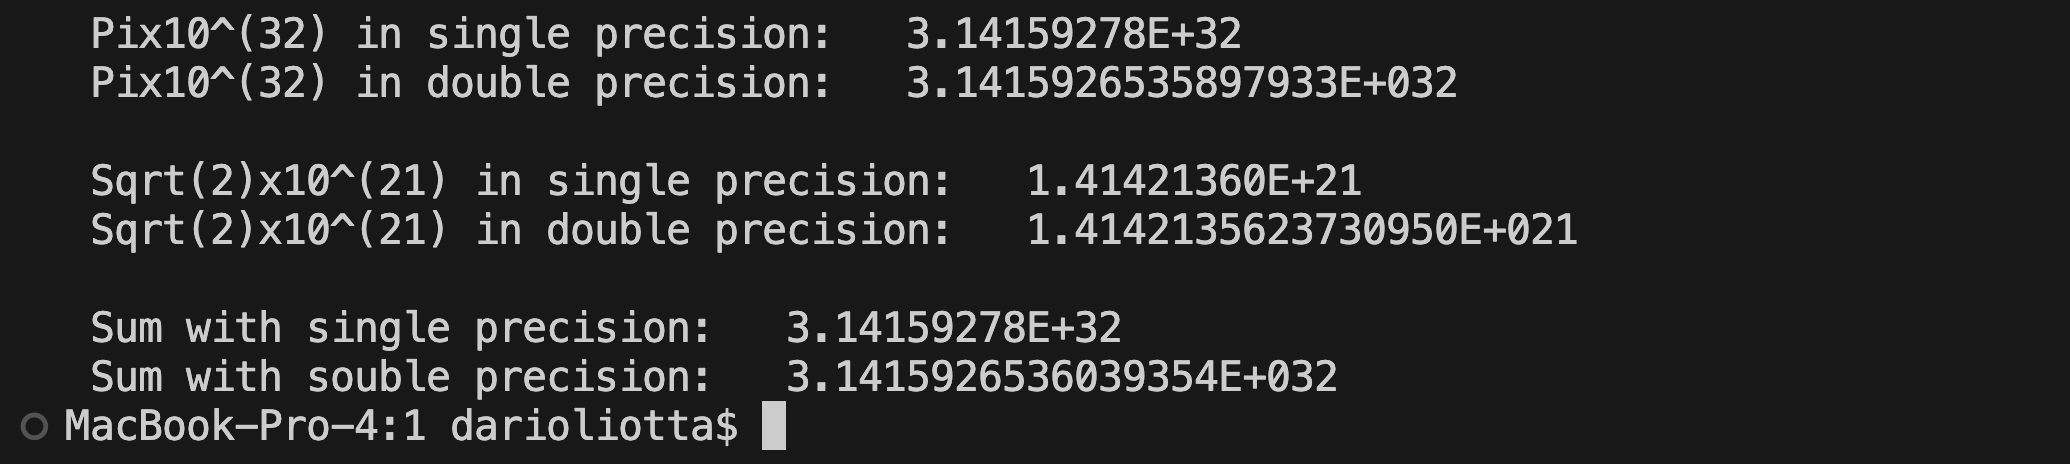
\includegraphics[width=0.78\textwidth]{Immagini/real-sum-output.png}
      \end{figure}

   \end{minipage}
\end{frame}

\section{Testing performance}

\begin{frame}
   \frametitle{Matrix-matrix multiplication: different approaches}

   \begin{minipage}{0.45\textwidth}
      \begin{center}
         \small{\textcolor{BrickRed}{\textbf{Standard approach}}}

         \footnotesize{Fill by rows}

         \begin{figure}[H]
    \centering
    \begin{tikzpicture}[scale=1.2]
        \draw (-1.25,-0.5) -- (-1.25,0.5);
        \draw (-1.25,-0.5) -- (-1.15,-0.5);
        \draw (-1.25,0.5) -- (-1.15,0.5);
        \draw (-0.25,-0.5) -- (-0.25,0.5);
        \draw (-0.25,-0.5) -- (-0.35,-0.5);
        \draw (-0.25,0.5) -- (-0.35,0.5);

        \node at (0,0) () {$\times$}; 

        \draw (1.25,-0.5) -- (1.25,0.5);
        \draw (1.25,-0.5) -- (1.15,-0.5);
        \draw (1.25,0.5) -- (1.15,0.5);
        \draw (0.25,-0.5) -- (0.25,0.5);
        \draw (0.25,-0.5) -- (0.35,-0.5);
        \draw (0.25,0.5) -- (0.35,0.5);

        \node at (1.5,0) () {$=$};

        \draw (2.75,-0.5) -- (2.75,0.5);
        \draw (2.75,-0.5) -- (2.65,-0.5);
        \draw (2.75,0.5) -- (2.65,0.5);
        \draw (1.75,-0.5) -- (1.75,0.5);
        \draw (1.75,-0.5) -- (1.85,-0.5);
        \draw (1.75,0.5) -- (1.85,0.5);

        \draw[color=BrickRed, ->] (-1.15,0.45) -- (-0.35,0.45);
        \draw[color=NavyBlue, ->] (-1.15,0.41) -- (-0.35,0.41);
        \node at (0.835,0) () {\scriptsize{...}};
        \draw[color=ForestGreen, ->] (-1.15,0.32) -- (-0.35,0.32);

        \draw[color=BrickRed] (0.4,-0.45) rectangle (0.5,0.45);
        \draw[color=NavyBlue] (0.57,-0.45) rectangle (0.67,0.45);
        \draw[color=ForestGreen] (1,-0.45) rectangle (1.1,0.45);

        \draw[color=BrickRed] (1.9,0.35) rectangle (2,0.45);
        \draw[color=NavyBlue] (2.07,0.35) rectangle (2.17,0.45);
        \node at (2.335,0.4) () {\scriptsize{...}};
        \draw[color=ForestGreen] (2.5,0.35) rectangle (2.6,0.45);
    \end{tikzpicture}
\end{figure}

         \vspace{-0.2cm}

         \begin{figure}[H]
            \centering
            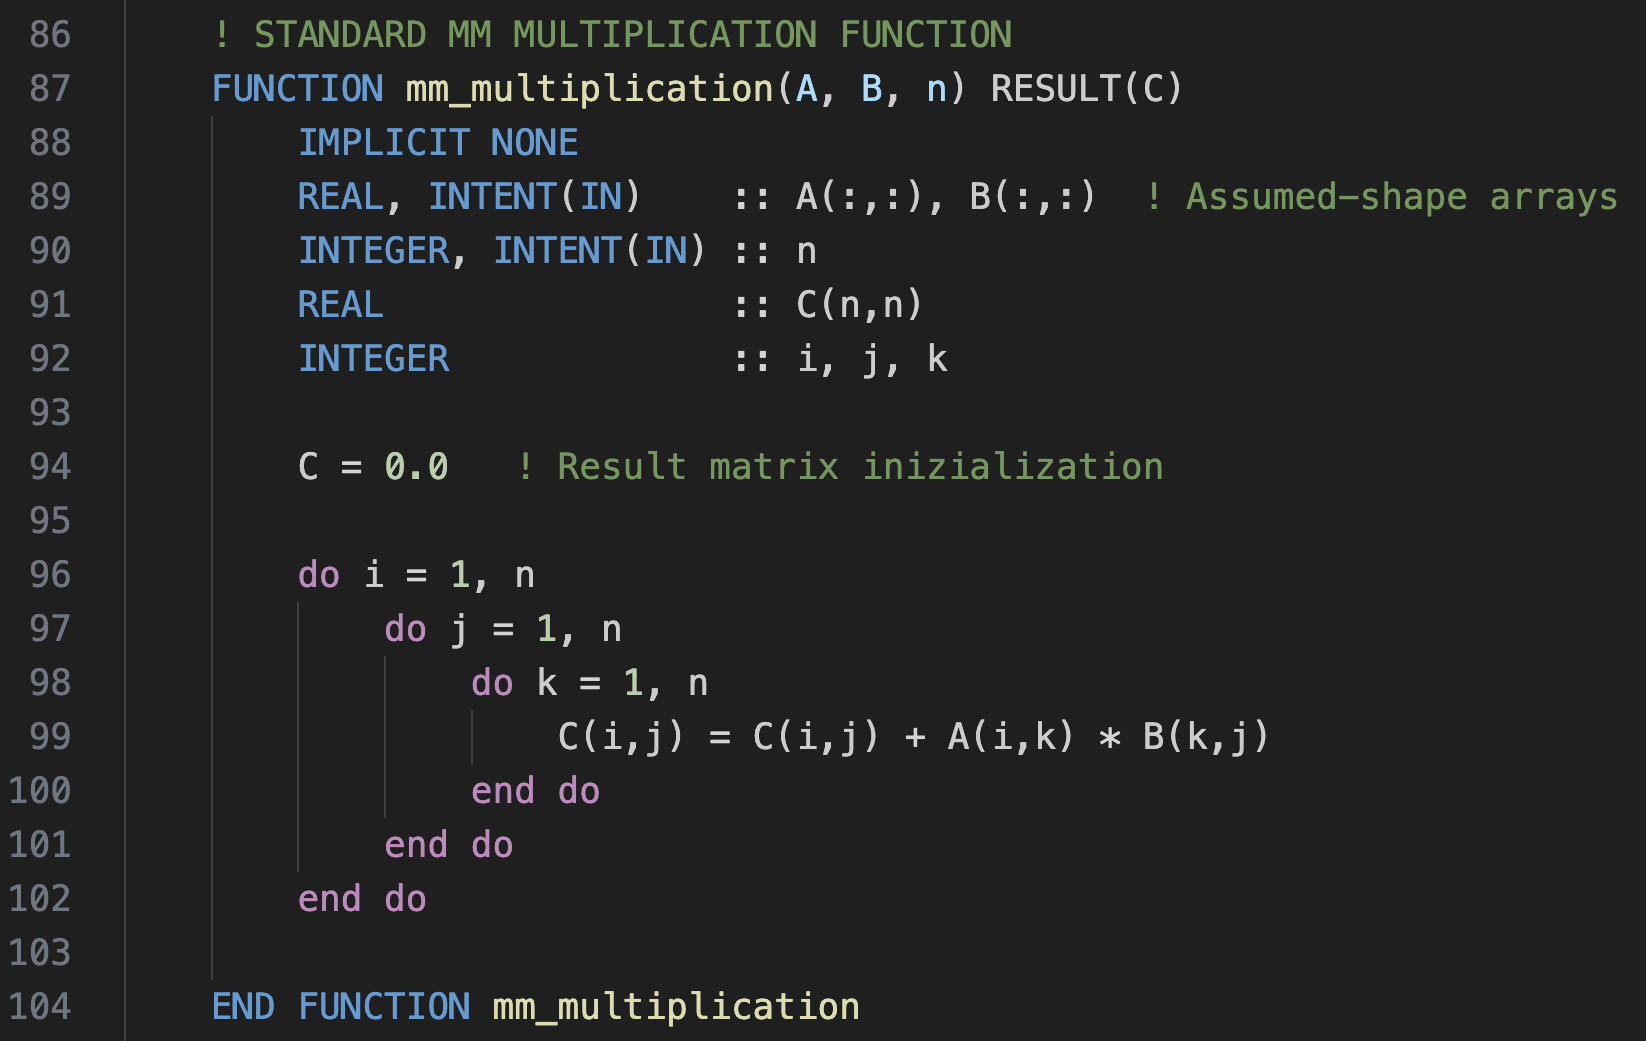
\includegraphics[width=0.8\textwidth]{Immagini/mm-multiplication-standard-code.png}
         \end{figure}

      \end{center}
   \end{minipage}
   \hfill
   \begin{minipage}{0.45\textwidth}
      \begin{center}
         \small{\textcolor{BrickRed}{\textbf{Reversed approach}}}

         \footnotesize{Fill by columns}

         \begin{figure}[H]
    \centering
    \begin{tikzpicture}[scale=1.2]
        \draw (-1.25,-0.5) -- (-1.25,0.5);
        \draw (-1.25,-0.5) -- (-1.15,-0.5);
        \draw (-1.25,0.5) -- (-1.15,0.5);
        \draw (-0.25,-0.5) -- (-0.25,0.5);
        \draw (-0.25,-0.5) -- (-0.35,-0.5);
        \draw (-0.25,0.5) -- (-0.35,0.5);

        \node at (0,0) () {$\times$}; 

        \draw (1.25,-0.5) -- (1.25,0.5);
        \draw (1.25,-0.5) -- (1.15,-0.5);
        \draw (1.25,0.5) -- (1.15,0.5);
        \draw (0.25,-0.5) -- (0.25,0.5);
        \draw (0.25,-0.5) -- (0.35,-0.5);
        \draw (0.25,0.5) -- (0.35,0.5);

        \node at (1.5,0) () {$=$};

        \draw (2.75,-0.5) -- (2.75,0.5);
        \draw (2.75,-0.5) -- (2.65,-0.5);
        \draw (2.75,0.5) -- (2.65,0.5);
        \draw (1.75,-0.5) -- (1.75,0.5);
        \draw (1.75,-0.5) -- (1.85,-0.5);
        \draw (1.75,0.5) -- (1.85,0.5);

        \draw[color=BrickRed, ->] (-1.15,0.45) -- (-1.15,-0.45);
        \draw[color=NavyBlue, ->] (-1.11,0.45) -- (-1.11,-0.45);
        \draw[color=ForestGreen, ->] (-1.05,0.45) -- (-1.05,-0.45);

        \draw[color=BrickRed] (0.4,0.35) rectangle (0.5,0.45);
        \draw[color=NavyBlue] (0.4,0.18) rectangle (0.5,0.28);
        \node[rotate=90] at (0.45,-0.085) () {\scriptsize{...}};
        \draw[color=ForestGreen] (0.4,-0.45) rectangle (0.5,-0.35);

        \draw[color=BrickRed, ->] (1.85,0.45) -- (1.85,-0.45);
        \draw[color=NavyBlue, ->] (1.89,0.45) -- (1.89,-0.45);
        \draw[color=ForestGreen, ->] (1.95,0.45) -- (1.95,-0.45);
    \end{tikzpicture}
\end{figure}

         \vspace{-0.2cm}

         \begin{figure}[H]
            \centering
            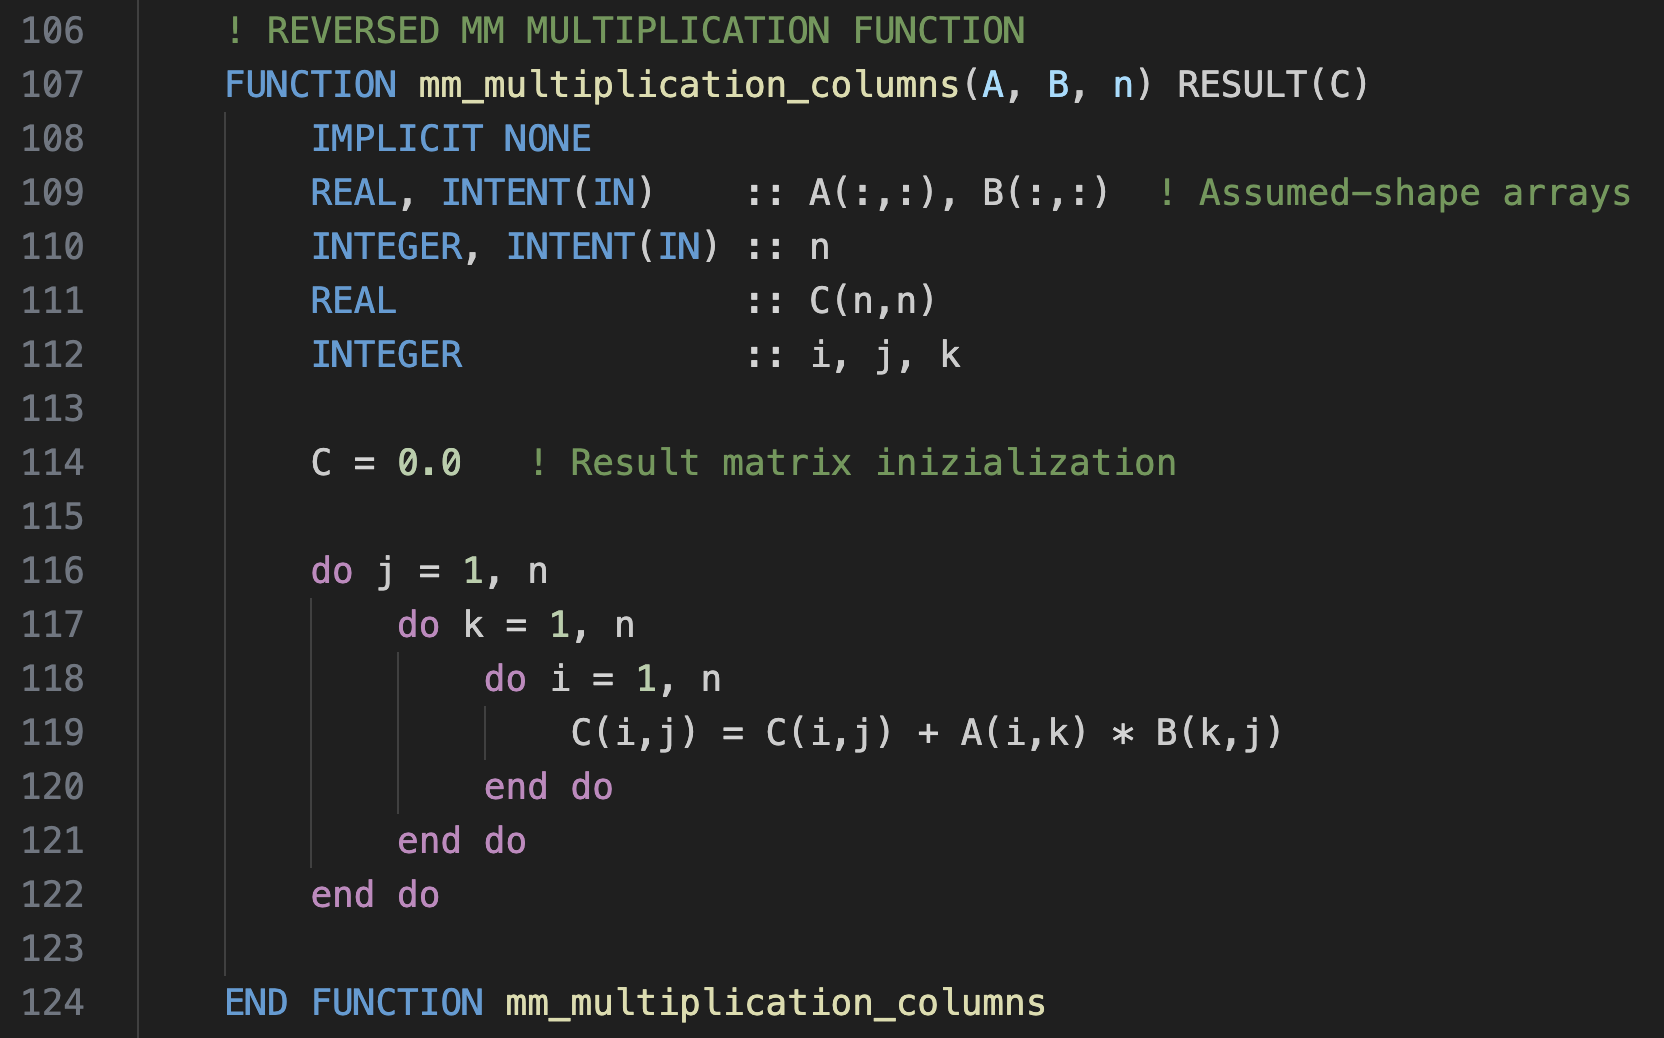
\includegraphics[width=0.8\textwidth]{Immagini/mm-multiplication-reversed-code.png}
         \end{figure}

      \end{center}
   \end{minipage}

   \vfill

   \begin{center}
      \small{\textcolor{BrickRed}{\textbf{Fortran approach}}}

      \footnotesize{Built-in function}

      \footnotesize{\texttt{REAL :: A(n,n), B(n,n), C(n,n)} $\ \ \Longrightarrow \ \ $ \texttt{C = \textcolor{BrickRed}{MATMUL(}A,B\textcolor{BrickRed}{)}}}
   \end{center}
\end{frame}

\begin{frame}
   \frametitle{Results with different input sizes}

   \begin{minipage}{0.45\textwidth}

      \vspace{0.25cm}

      \begin{itemize}
         \small{\item $10$ different \textcolor{BrickRed}{\textbf{input sizes}}}
         \small{\item $10$ \textcolor{BrickRed}{\textbf{runs}} for each size}
         \small{\item Times evaluated with function \textcolor{BrickRed}{\texttt{\textbf{CPU\_TIME()}}}}
         \small{\item Final times are the \textcolor{BrickRed}{\textbf{average}} ones elapsed for each run}
      \end{itemize}

      \begin{figure}[H]
         \centering
            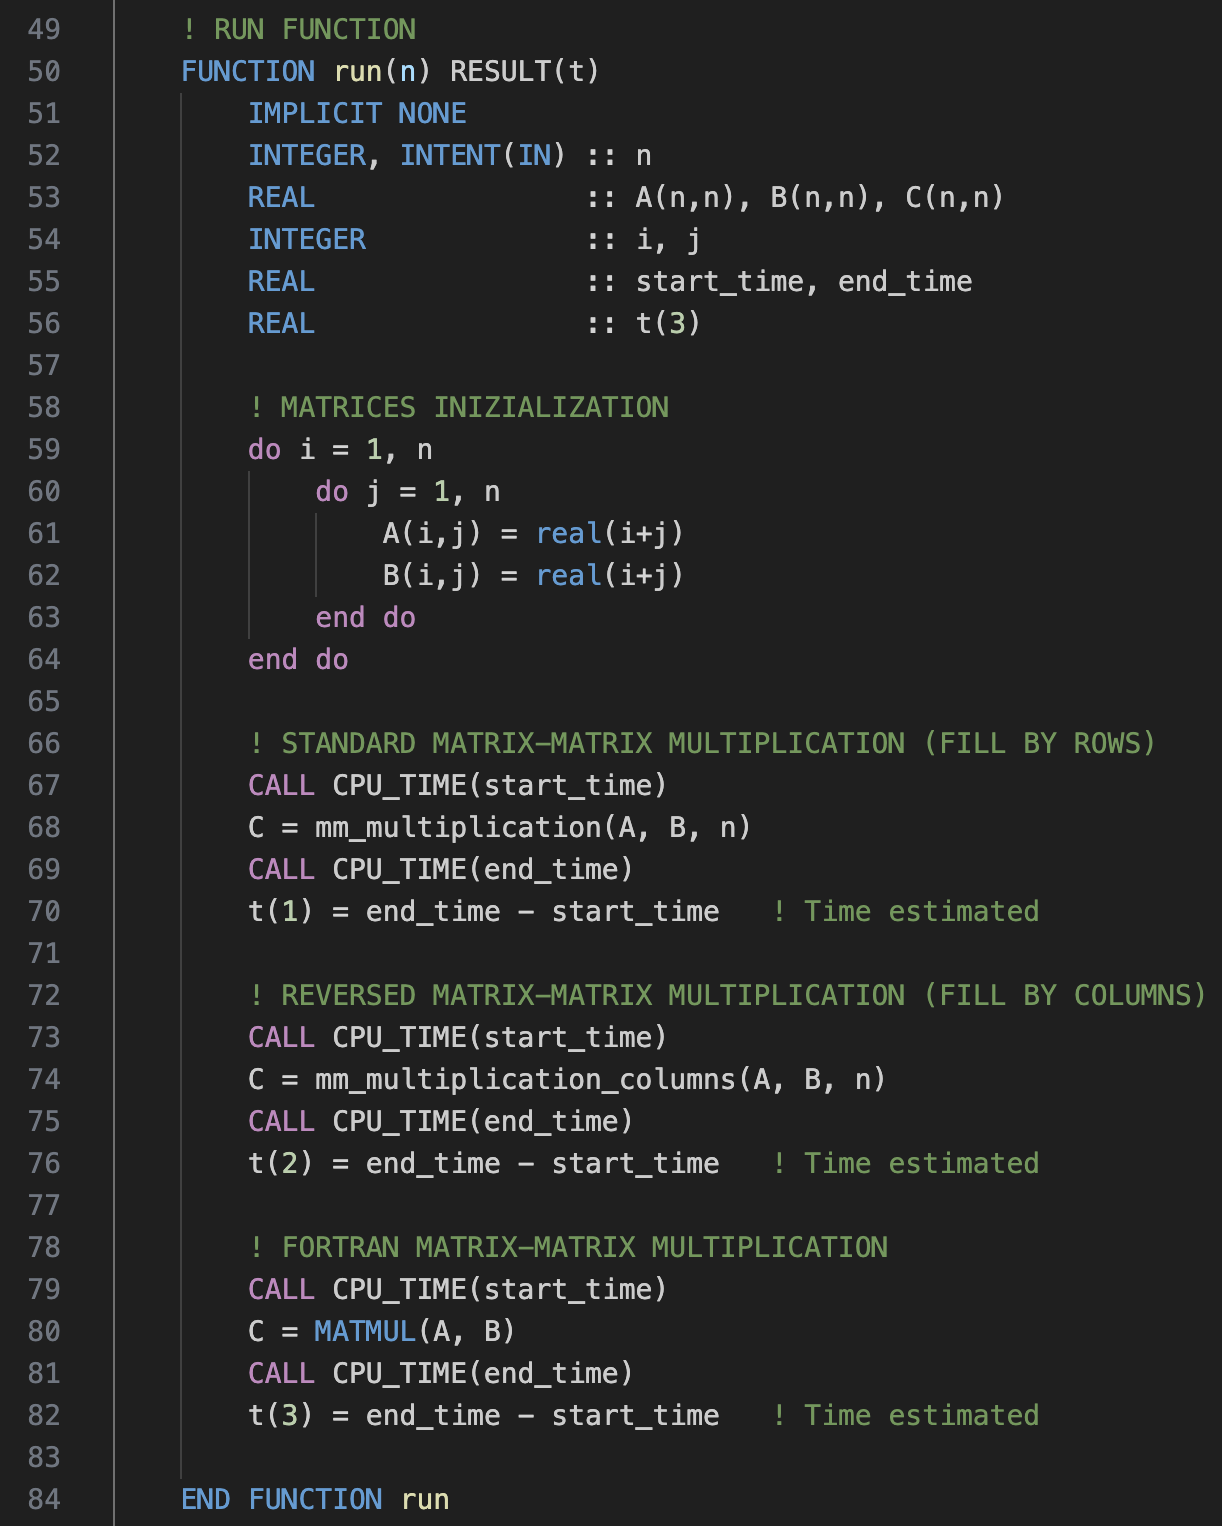
\includegraphics[width=0.57\textwidth]{Immagini/run-function.png}
            \caption*{\tiny{\textbf{Run function}}}
      \end{figure}
   \end{minipage}
   \hfill
   \begin{minipage}{0.5\textwidth}
      \begin{figure}[H]
         \centering
            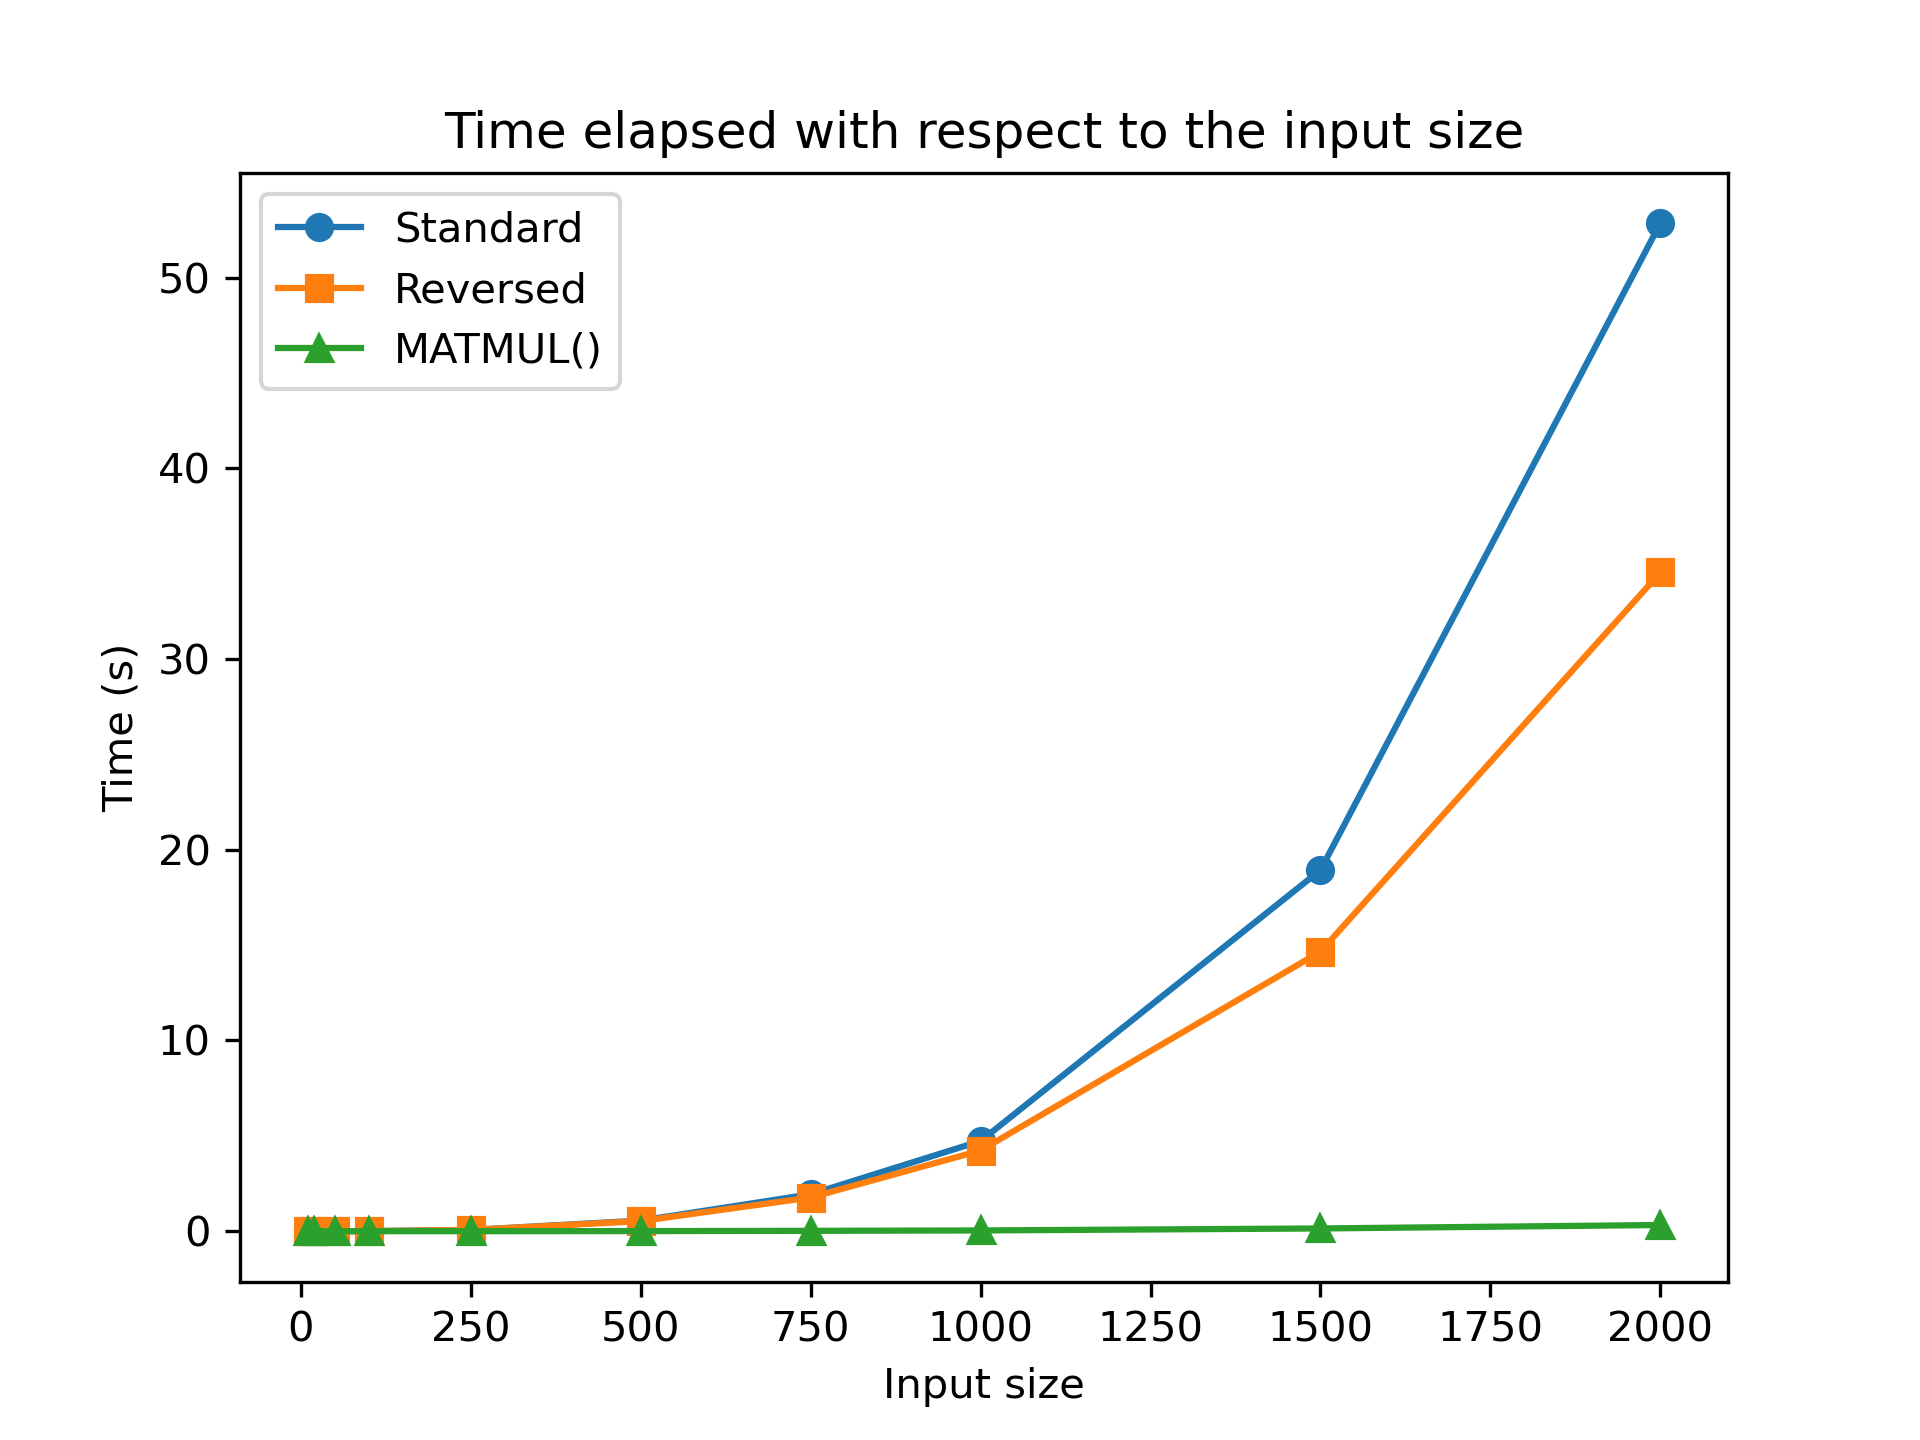
\includegraphics[width=0.92\textwidth]{Immagini/plot_t_sum.png}
      \end{figure}

      \vspace{-0.15cm}

      \begin{itemize}
         \small{\item Standard approach is the worst}
         \small{\item Reversed approach is better, probably because of the \textcolor{BrickRed}{\textbf{column-major memory layout}} (cache optimization)}
         \small{\item \texttt{MATMUL()} function is the best, since it's an \textcolor{BrickRed}{\textbf{intrinsic function}}} 
      \end{itemize}

      \vfill
   \end{minipage}
\end{frame}

\begin{frame}
   \frametitle{Results with different optimizations}

   \tiny

   \begin{table}[H]
      \centering
      \begin{tabular}{l l}
         \textbf{Flag} & \textbf{Description}\\
         \hline
         \texttt{-O0} & No optimization\\
         \hline
         \texttt{-O1} & Base optimization; reduces code dimensions and improves performances\\
         \hline
         \texttt{-O2} & Aggressive optimization; enables further options without time compilation increases\\
         \hline
         \texttt{-O3} & Maximum optimization; includes advanced optimization such as unrolling of cycles\\
         \hline
         \texttt{-march=native} & Optimizes code for the CPU architecture where it is compiled\\
         \hline
         \texttt{-funroll-loops} & Unrolls loops to improve performances
      \end{tabular}
   \end{table}

   \begin{minipage}{0.32\textwidth}
      \begin{center}
         \small{\textcolor{BrickRed}{\textbf{Standard approach}}}
      \end{center}
      \vspace{-0.5cm}
      \begin{figure}[H]
         \centering
         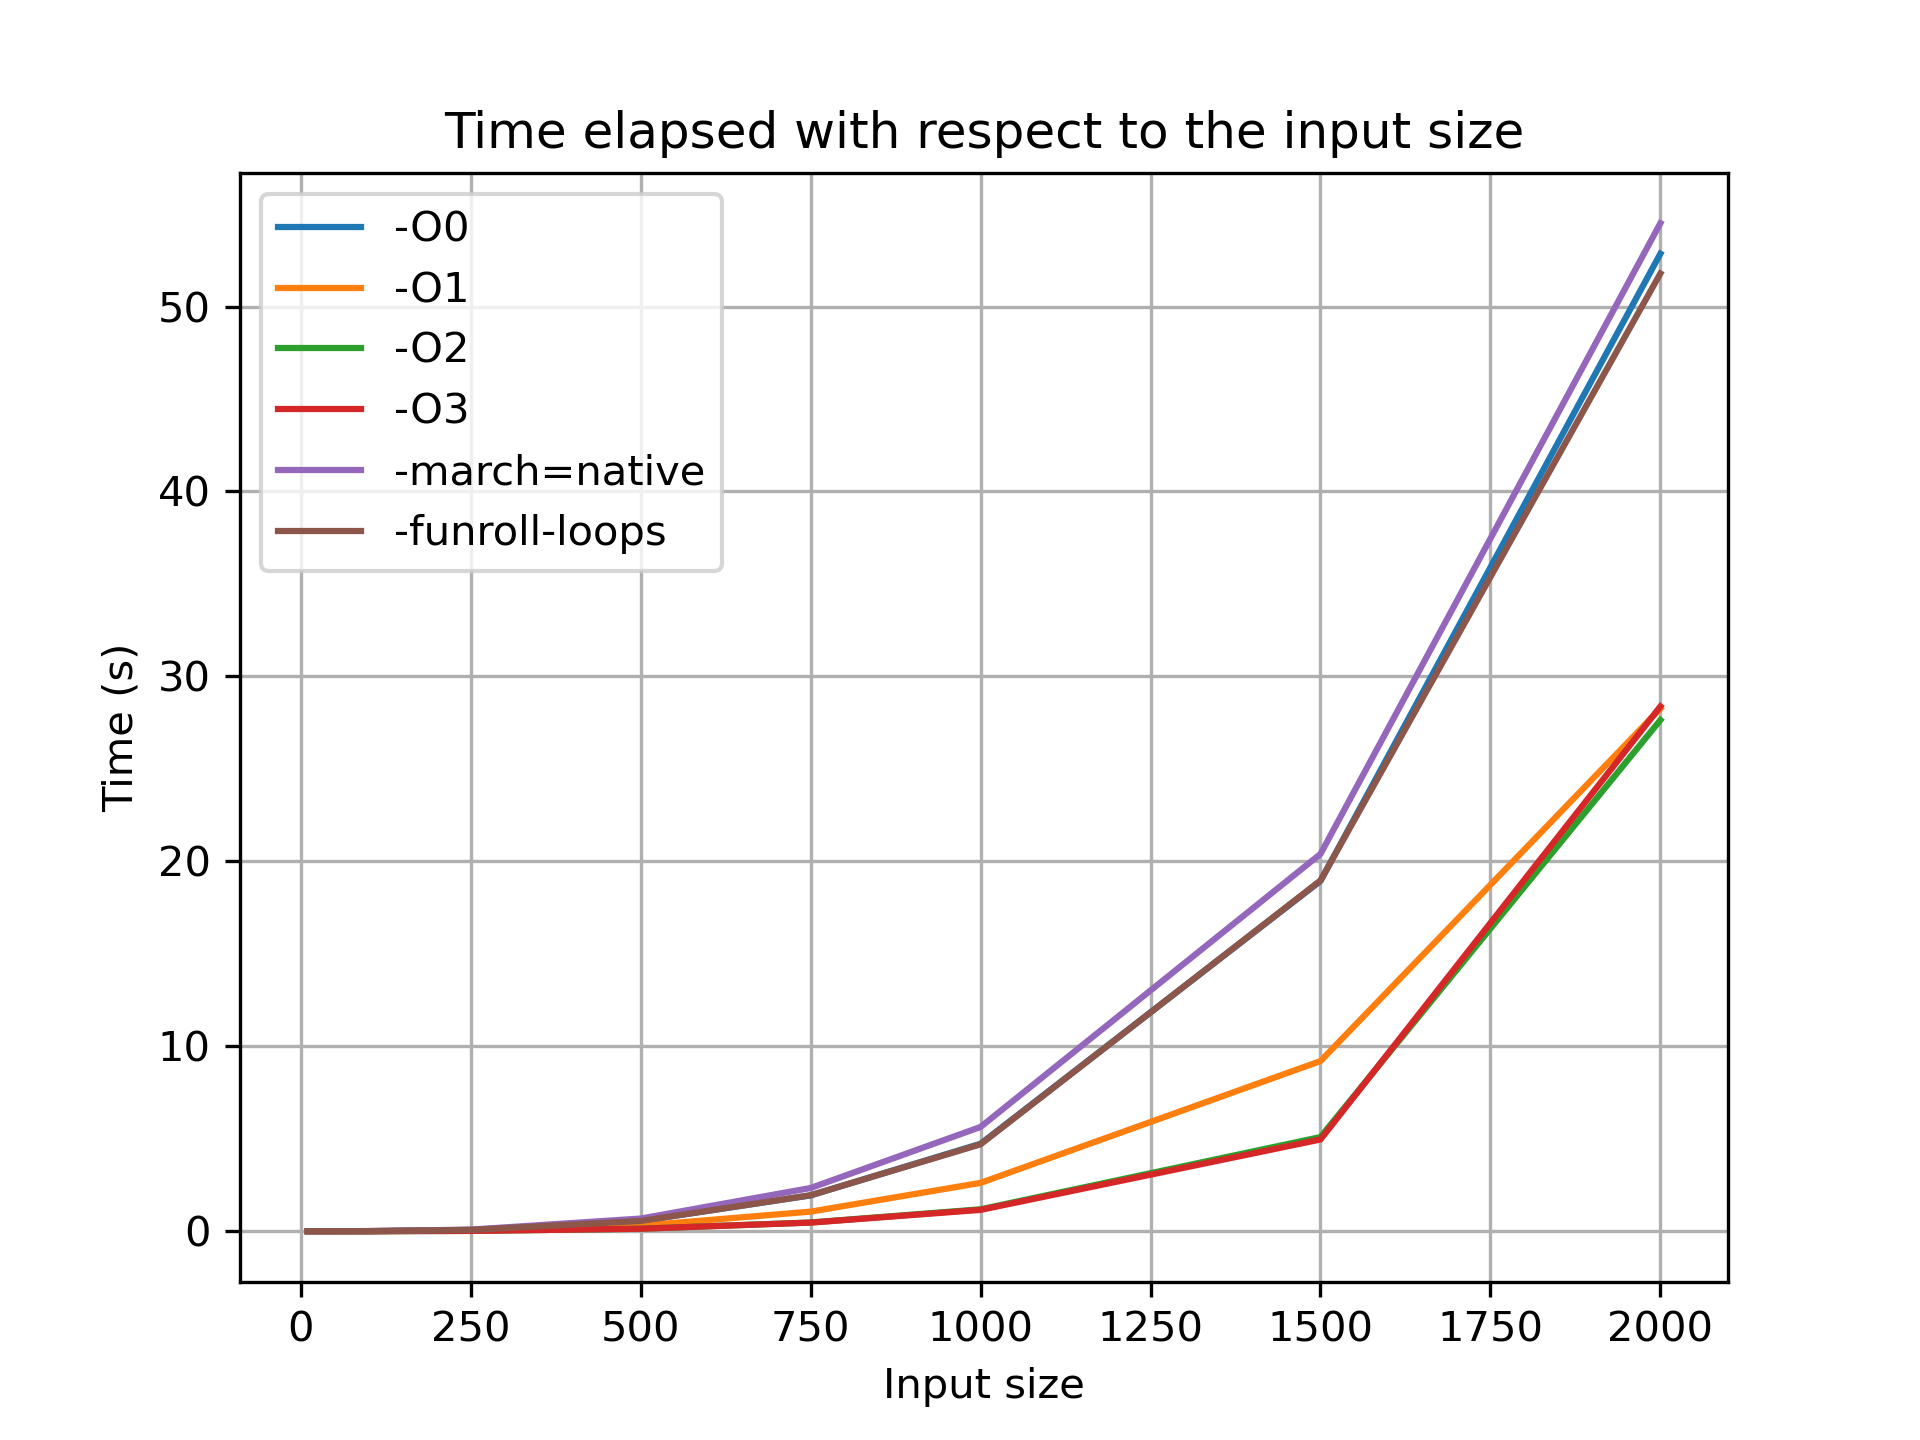
\includegraphics[width=\textwidth]{Immagini/plot_t_sum_standard.png}
      \end{figure}
   \end{minipage}
   \hfill
   \begin{minipage}{0.32\textwidth}
      \begin{center}
         \small{\textcolor{BrickRed}{\textbf{Reversed approach}}}
      \end{center}
      \vspace{-0.5cm}
      \begin{figure}[H]
         \centering
         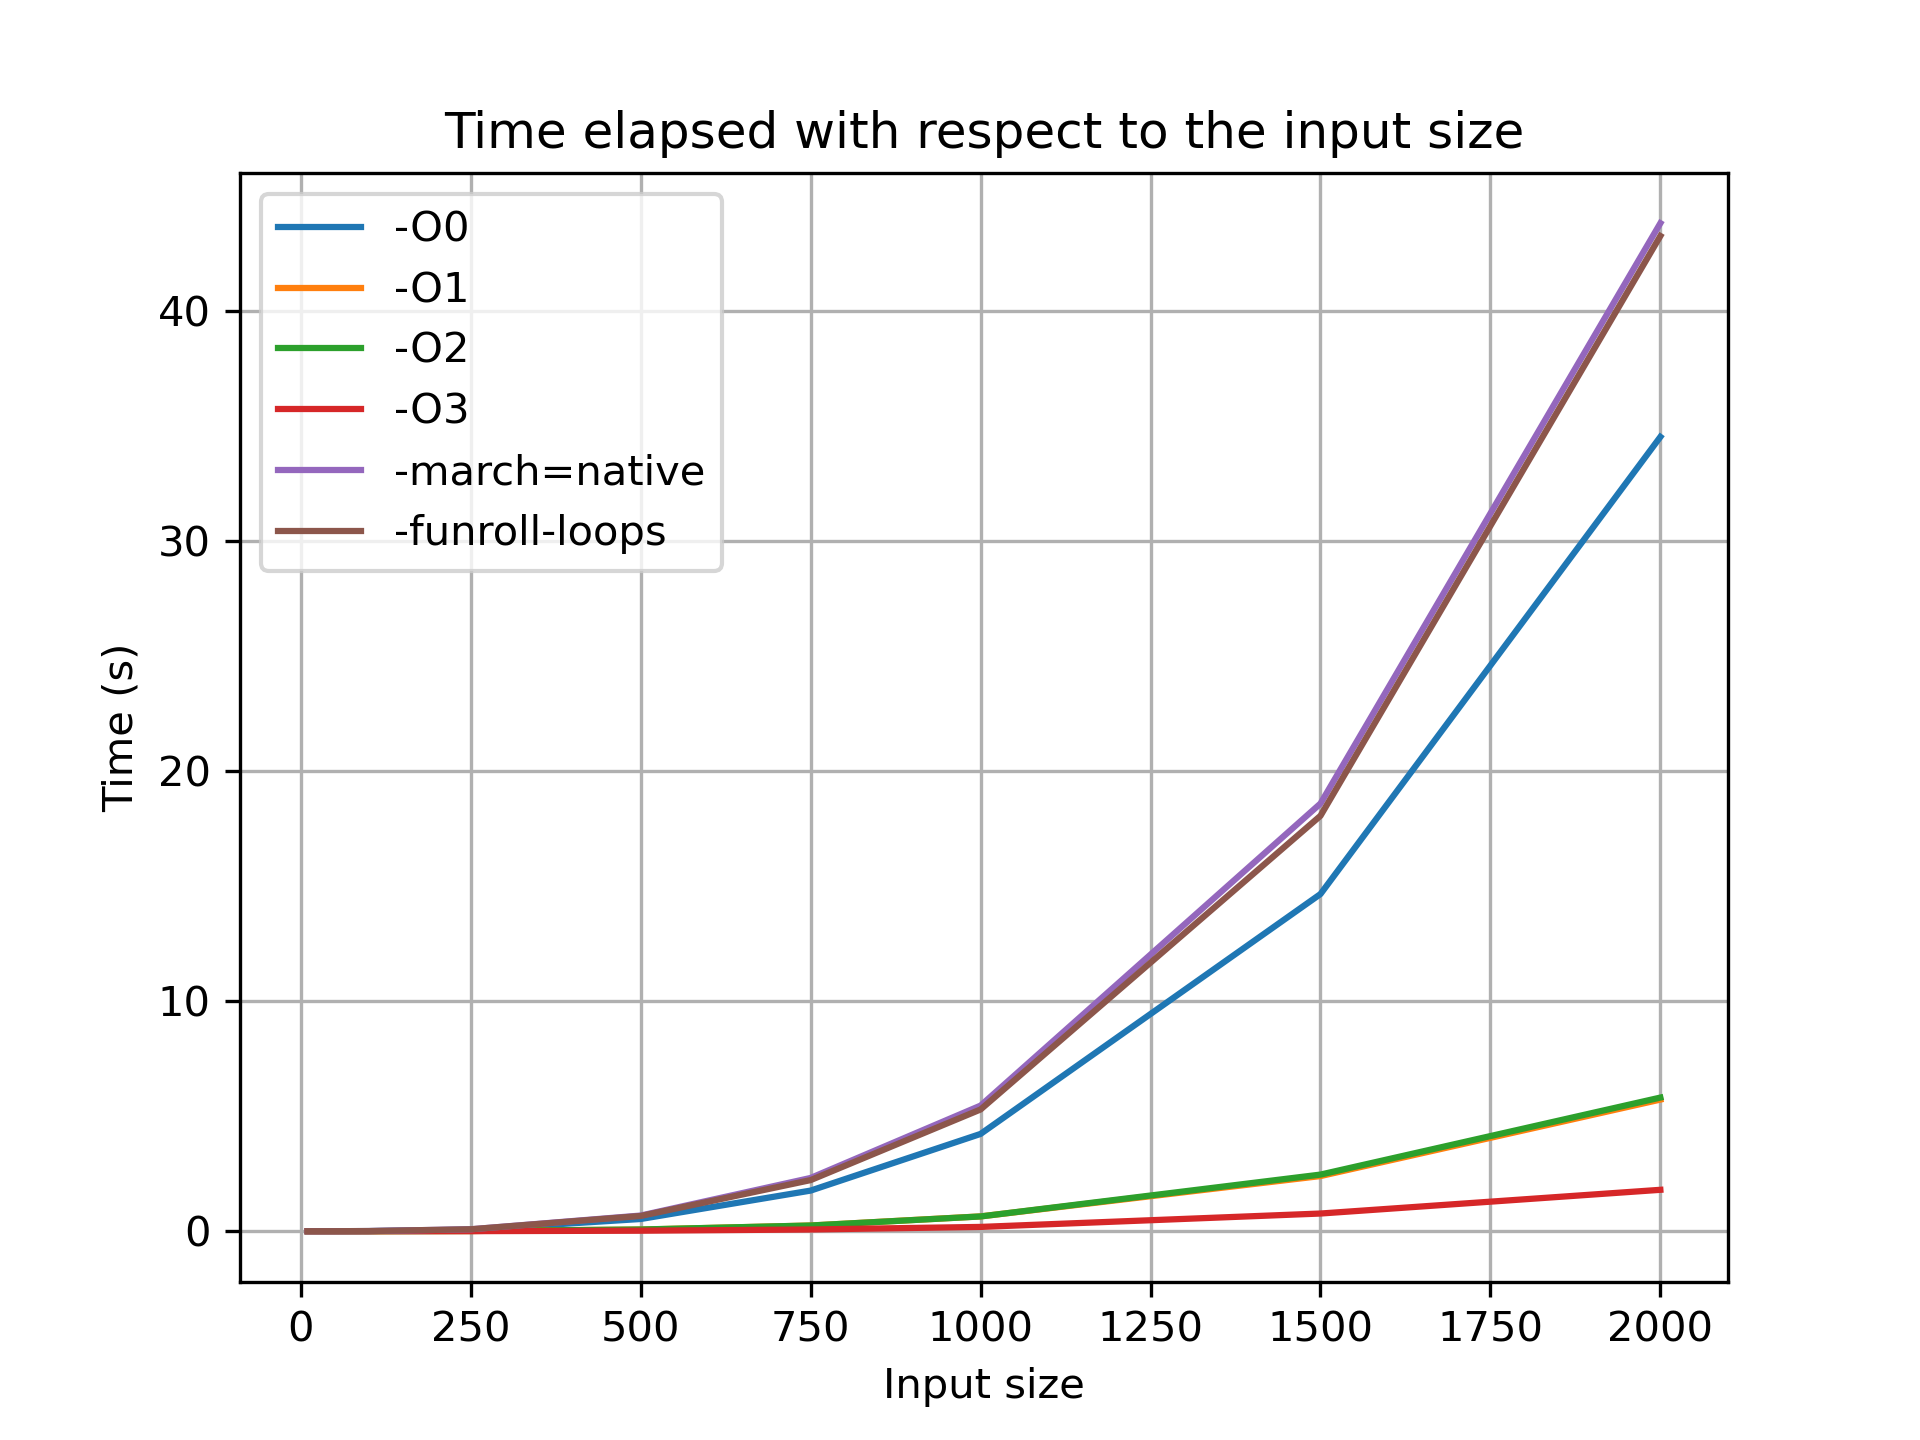
\includegraphics[width=\textwidth]{Immagini/plot_t_sum_reversed.png}
      \end{figure}
   \end{minipage}
   \hfill
   \begin{minipage}{0.32\textwidth}
      \begin{center}
         \small{\textcolor{BrickRed}{\textbf{Fortran approach}}}
      \end{center}
      \vspace{-0.5cm}
      \begin{figure}[H]
         \centering
         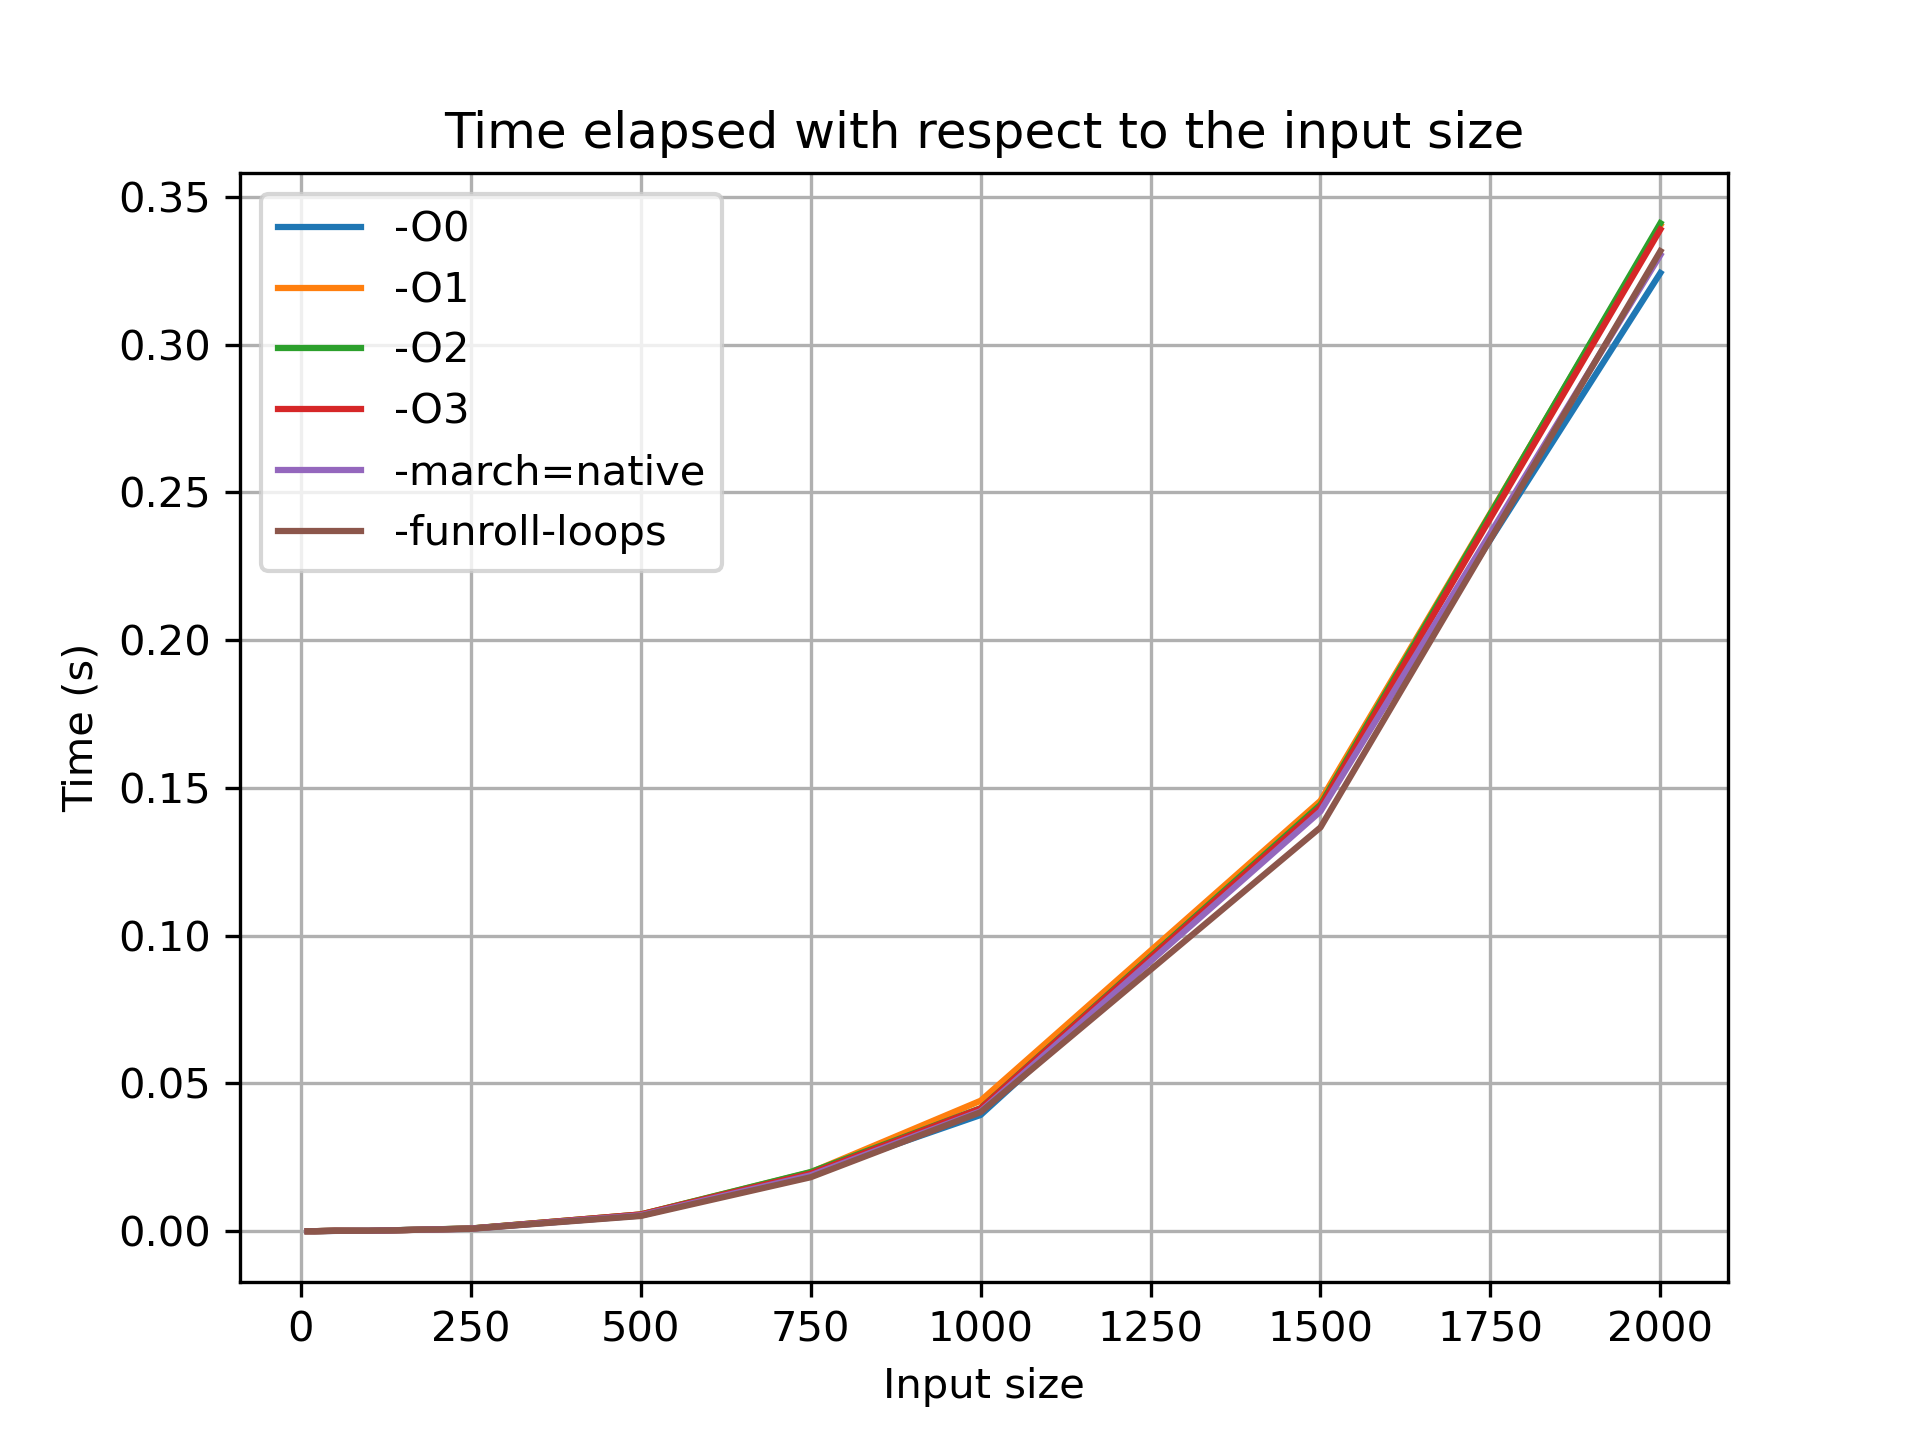
\includegraphics[width=\textwidth]{Immagini/plot_t_sum_fortran.png}
      \end{figure}
   \end{minipage}

   \vfill

   \begin{itemize}
      \footnotesize{\item The only difference appeare to be made by \texttt{-O1}, \texttt{-O2} and \texttt{-O3}, both for the \textbf{standard} and the \textbf{reversed} approach (approximately half of the time)}
      \footnotesize{\item All optimization are similar in the \textbf{fortran} approach, as it is already much optimized}
   \end{itemize}
\end{frame}

\end{document}